\documentclass[]{article}
\usepackage{lmodern}
\usepackage{amssymb,amsmath}
\usepackage{ifxetex,ifluatex}
\usepackage{fixltx2e} % provides \textsubscript
\ifnum 0\ifxetex 1\fi\ifluatex 1\fi=0 % if pdftex
  \usepackage[T1]{fontenc}
  \usepackage[utf8]{inputenc}
\else % if luatex or xelatex
  \ifxetex
    \usepackage{mathspec}
  \else
    \usepackage{fontspec}
  \fi
  \defaultfontfeatures{Ligatures=TeX,Scale=MatchLowercase}
\fi
% use upquote if available, for straight quotes in verbatim environments
\IfFileExists{upquote.sty}{\usepackage{upquote}}{}
% use microtype if available
\IfFileExists{microtype.sty}{%
\usepackage[]{microtype}
\UseMicrotypeSet[protrusion]{basicmath} % disable protrusion for tt fonts
}{}
\PassOptionsToPackage{hyphens}{url} % url is loaded by hyperref
\usepackage[unicode=true]{hyperref}
\hypersetup{
            pdfborder={0 0 0},
            breaklinks=true}
\urlstyle{same}  % don't use monospace font for urls
\usepackage{graphicx,grffile}
\makeatletter
\def\maxwidth{\ifdim\Gin@nat@width>\linewidth\linewidth\else\Gin@nat@width\fi}
\def\maxheight{\ifdim\Gin@nat@height>\textheight\textheight\else\Gin@nat@height\fi}
\makeatother
% Scale images if necessary, so that they will not overflow the page
% margins by default, and it is still possible to overwrite the defaults
% using explicit options in \includegraphics[width, height, ...]{}
\setkeys{Gin}{width=\maxwidth,height=\maxheight,keepaspectratio}
\IfFileExists{parskip.sty}{%
\usepackage{parskip}
}{% else
\setlength{\parindent}{0pt}
\setlength{\parskip}{6pt plus 2pt minus 1pt}
}
\setlength{\emergencystretch}{3em}  % prevent overfull lines
\providecommand{\tightlist}{%
  \setlength{\itemsep}{0pt}\setlength{\parskip}{0pt}}
\setcounter{secnumdepth}{0}
% Redefines (sub)paragraphs to behave more like sections
\ifx\paragraph\undefined\else
\let\oldparagraph\paragraph
\renewcommand{\paragraph}[1]{\oldparagraph{#1}\mbox{}}
\fi
\ifx\subparagraph\undefined\else
\let\oldsubparagraph\subparagraph
\renewcommand{\subparagraph}[1]{\oldsubparagraph{#1}\mbox{}}
\fi

% set default figure placement to htbp
\makeatletter
\def\fps@figure{htbp}
\makeatother


\date{}

\begin{document}

\subsection{The Mission: Industrialize
Luna}\label{the-mission-industrialize-luna}

This exercise follows Section H9 in the Colonization rules. The
difference is that I'm showing the initial research buildup, and using
different components.

\subsubsection{Year 1}\label{year-1}

\begin{itemize}
\tightlist
\item
  Operation: income 2, just because. (H1)
\end{itemize}

\subsubsection{Year 2}\label{year-2}

\begin{itemize}
\tightlist
\item
  Operation: research: acquire Photon Heliogyro for 0. (H2)
\end{itemize}

\subsubsection{Year 3}\label{year-3}

\begin{itemize}
\tightlist
\item
  Operation: sell Photon Heliogyro for 5 WT. (H3)
\end{itemize}

\subsubsection{Year 4}\label{year-4}

\begin{itemize}
\tightlist
\item
  Operation: research: acquire Pondermotive VASIMR (H2). What does the
  Yellow signify?
\end{itemize}

Apparently this thruster is ``pushable;'' cursory examination of the
rules reveals I don't care about pushability right now. Cost 0. (H2)

\subsubsection{Year 5}\label{year-5}

\begin{itemize}
\tightlist
\item
  Operation: research: acquire Tungsten Resistojet, cost 0, mass 2. (H2)
\end{itemize}

\begin{figure}
\centering
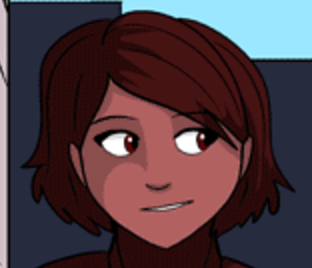
\includegraphics{images/bubbles-smiles.png}
\caption{Bubbles smiles}
\end{figure}

\subsubsection{Year 6}\label{year-6}

\begin{itemize}
\tightlist
\item
  Operation: boost crew, thruster and robonaut to LEO stack; Dry Mass 6.
  (H4)
\end{itemize}

\begin{enumerate}
\def\labelenumi{\arabic{enumi}.}
\item
  Free Action: Cargo Transfer: Form rocket from current LEO stack, mass
\item
  Net Thrust is 5.
\item
  Free Action: Fuel up, 5 WT, moves fuel figure (wet mass) to 11, Net
  Thrust: 4.
\item
  Move: move rocket from LEO, burn 4 to get into HEO. Wet mass 9.
\item
  Free Action(?): Switch to crew thruster.
\item
  Free Action: jettison Tungsten Resistojet, Dry Mass now 3, Wet Mass
\item
  (D1.5)
\item
  Free Action: decommission Tungsten Resistojet. (D1.6)
\end{enumerate}

\subsubsection{Year 7}\label{year-7}

\begin{enumerate}
\def\labelenumi{\arabic{enumi}.}
\tightlist
\item
  Move: land on moon, 1 burn, 8 steps, Wet Mass now 3 \& 1/2. (G1)
\end{enumerate}

\begin{itemize}
\tightlist
\item
  Operation: prospect the site, which fails because the Tungsten
  Resistojet has ISRU 3, and there are only two hydrations. Bummer. (H6)
\end{itemize}

If we ditch the robonaut, we can get to DM 1, WM 1 \& 3/7, not enough to
boost. So we need to mine fuel in-situ, which is an operation.

\subsubsection{Year 8}\label{year-8}

\begin{itemize}
\tightlist
\item
  ISRU for fuel. The ISRU rating of the Tungsten Resistojet is 3. The
  yield on Luna is 2. Looks like crew is stranded on Luna: 1 + 2 - 3 =
  0.
\end{itemize}

No fuel for you! (H5)

Ok, that was interesting. I think I'm getting a feeling why this game
could get very addictive very quickly.

\end{document}
